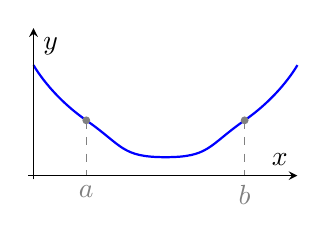
\begin{tikzpicture}
    \begin{axis}[
        axis lines = middle,
        axis on top,
        clip = false,
        xlabel = $x$,
        ylabel = {$y$},
        xtick = \empty,
        ytick = \empty,
        xmin=-0.1,xmax=5,
        ymin=-0.1,ymax=4,
        width=5cm,
        height=3.5cm
    ]
    
       % Define points
    \coordinate (A) at (0,3);
    \coordinate (B) at (1,1.5);
    \coordinate (C) at (2.5,0.5);
    \coordinate (D) at (4,1.5);
    \coordinate (E) at (5,3);

    \coordinate (Ax) at (0,0);
    \coordinate (Bx) at (1,0.0);
    \coordinate (Cx) at (2.5,0.0);
    \coordinate (Dx) at (4,0.0);
    \coordinate (Ex) at (5,0);

    % Draw smooth curve through the points
    \draw [blue, thick] plot[smooth, tension=1] coordinates {(A) (B) (C) (D) (E)};
    
    % Draw points for reference
    \draw[gray, dashed] (B) node[circle, fill=gray, inner sep=1pt] {} -- (Bx)   node[at end, below] {$a$};
    \draw[gray, dashed] (D) node[circle, fill=gray, inner sep=1pt] {} -- (Dx)   node[at end, below] {$b$};
    
    \end{axis}
    \end{tikzpicture}
